\pagebreak
\section{Fallschirmjäger}

\subsection{Fahrzeuge}
\begin{longtable}{lcccc} 
	\toprule
	Typ & C-130 & CH-47 &	Huron	&	Mohawk \\ 
	\midrule
	Passagiere 	&	25 	&	25 	&	18 	&	16 \\ 
	Min. Sprunghöhe	& 500\,m 	& 300\,m 	&	300\,m	&	300\,m	\\
	Max. Sprunghöhe	&	1000\,m 	&	500\,m 	&	500\,m	&	500\,m \\
	Min. Geschwindigkeit	& 	200\,km/h	&	120\,km/h	&	120\,km/h	&	120\,km/h	\\ 
	Max. Geschwindigkeit	& 	250\,km/h	&	150\,km/h &	150\,km/h &	150\,km/h \\
	\bottomrule 
\end{longtable}

\subsection{Sprungvorbereitung}
\subsubsection*{Kartenvorbereitung}
\begin{tabular}{C{0.1\linewidth}m{0.2\linewidth} m{0.65\linewidth}}
	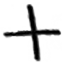
\includegraphics[scale=0.8]{./img/fortgeschrittenes/fallschirmspringen/sammelzone}	& Sammelzone (SZ)	& ist der Punkt wo sich ein Trupp sammelt, es werden immer 2 Sammelzonen pro Trupp bestimmt\\
	
\includegraphics[scale=0.8]{./img/fortgeschrittenes/fallschirmspringen/wendepunkt} 	& 	Wendepunkt (WP) & Pilot übergibt Loadmaster Befehlsgewalt, letzte Vorbereitung vor Sprung\\
	
\includegraphics[scale=0.8]{./img/fortgeschrittenes/fallschirmspringen/dropzone}	& Dropzone (DZ) & ab hier beginnt der Loadmaster mit dem Sprung
\end{tabular}

\subsubsection*{Materialvorbereitung\,/\,Aufsitzen}
\begin{enumerate}
	\item Rucksack auf den Bauch schnallen 
	\item Fallschirm sowie Höhenmesser aus der speziellen Kiste entnehmen
	\item im Trupp vor der Maschine aufstellen; der Loadmaster ist der letzte der einsteigt
	\item im Fahrzeug den Höhenmesser aktivieren \keys{O}\ \underline{selbstständig} und \underline{ohne} Funkbestätigung auf die SR 200 (Sprungfrequenz) wechseln
	\item Truppführer meldet aufsitzen auf der SR 200
\end{enumerate}

\begin{flushright}
	Merke: >>Der Erste wird der Letzte sein.<< 
\end{flushright} 


\subsection{Loadmaster}
Der Loadmaster hat die primäre Aufgabe den Absprung in der Luft zu koordinieren, darunter fällt
zum Beispiel welcher Trupp springt zu welcher Zeit. Des weiteren wird nur auf sein Kommando
gesprungen.

\subsubsection*{Teil der Truppe}
	Die Rolle des Loadmasters wird von ein Mitglied des zuletzt springenden Trupps wahrgenommen.
	Der Loadmaster springt immer als letztes ab, egal welche Position er im Trupp hat.

\subsubsection*{Teil des Fahrzeugteams}
	Die Rolle des Loadmaster wird von einem dritten Mann im Fahrzeug wahrgenommen. Dieser springt am Ende nicht ab, sondern verbleibt im Fahrzeug.

\subsection{Der Sprung}
\subsubsection*{Verhalten beim Sprung}
	Der Fallschirm wird sofort nach Verlassen des Fahrzeuges geöffnet.
	
\subsubsection*{Besonderheiten von ACE3}
	Durch die Modifikation ACE3 kann es vorkommen, dass sich der Fallschirm nicht öffnet. Sollte dies der Fall sein, so muss man durch das ACE-Eigenmenü \keys{StrG+Win} den Fallschirm abschneiden. Anschließend kann man einen Reservefallschirm öffnen, dieser ist jedoch nicht steuerbar.

\subsection{Der Flug}
	Während des gesamten Fluges sollte man versuchen die maximal Geschwindigkeit von 9m/s zu halten, außerdem ist es hilfreich sich beim Navigieren an seinem Vordermann zu orientieren.

\subsection{Die Landung}
\begin{enumerate}
	\item beginnt ab einer Höhe von 50\,m; von da an beträgt die maximal Geschwindigkeit 5m/s,
	\item 20m vor der Landung auf mindestens 3\,m/s abbremsen,
	\item sollte mit maximal 2\,m/s oder weniger erfolgen um Verletzungen zu vermeiden.
\end{enumerate}

\subsection{Sammeln}
\begin{enumerate}
	\item Nach der Landung wird über den Truppfunk das erfolgreiche Landen gemeldet.
	\item Es wird sich eigenständig zur ersten Sammelzone begeben (dafür sind 5min vorgesehen).
	\item Wenn der Trupp vollständig an der ersten Sammelzone ist, bewegt sich dieser zur zweiten
	Sammelzone. Sollten es nicht alle Kameraden zur ersten Sammelzone schaffen bzw. sich
	nach der Landung nicht melden, wird die Suche nach den vermissten Kameraden
	aufgenommen.
	\item Beim Erreichen des zweiten Brückenkopfes ist der Fallschirmsprung abgeschlossen.
\end{enumerate}	